% Copyright © 2017-2018 Martin Ueding <dev@martin-ueding.de>
% Licensed under CC-BY 4.0

\documentclass{scrartcl}

\pagestyle{empty}

\usepackage{tikz}
\usetikzlibrary{arrows.meta, calc}

\begin{document}

\newcommand\boostfactorTwoD{0.3}
\newcommand\boostfactorThreeD{0.3}

No boost:

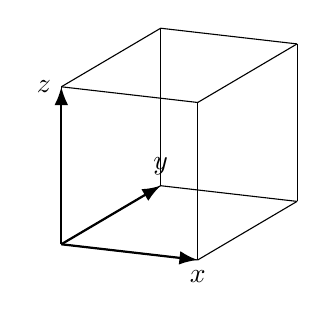
\begin{tikzpicture}[
        rotate around x=-90,
        rotate around z=-15,
        scale=2,
    ]

    \draw[thick, ->, >=Latex] (0, 0, 0) -- ++(1, 0, 0) node[below] {$x$};
    \draw[thick, ->, >=Latex] (0, 0, 0) -- ++(0, 1, 0) node[above] {$y$};
    \draw[thick, ->, >=Latex] (0, 0, 0) -- ++(0, 0, 1) node[left] {$z$};

    \coordinate (boostx) at (1, 0, 0);
    \coordinate (boosty) at (0, 1, 0);
    \coordinate (boostz) at (0, 0, 1);

    \foreach \a in {0,1}
    \foreach \b in {0,1}
    {
        \draw ($\a*(boostx) + \b*(boosty)$) -- ++(boostz);
        \draw ($\a*(boosty) + \b*(boostz)$) -- ++(boostx);
        \draw ($\a*(boostz) + \b*(boostx)$) -- ++(boosty);
    }
\end{tikzpicture}

\vspace{10ex}

Boost along the $(1, 1, 0)$ direction:

\begin{tikzpicture}[
        rotate around x=-90,
        rotate around z=-15,
        scale=2,
    ]

    \draw[thick, ->, >=Latex] (0, 0, 0) -- ++(1, 0, 0) node[below] {$x$};
    \draw[thick, ->, >=Latex] (0, 0, 0) -- ++(0, 1, 0) node[above] {$y$};
    \draw[thick, ->, >=Latex] (0, 0, 0) -- ++(0, 0, 1) node[left] {$z$};

    \coordinate (boostx) at (1+\boostfactorTwoD, \boostfactorTwoD, 0);
    \coordinate (boosty) at (\boostfactorTwoD, 1+\boostfactorTwoD, 0);
    \coordinate (boostz) at (0, 0, 1);

    \foreach \a in {0,1}
    \foreach \b in {0,1}
    {
        \draw ($\a*(boostx) + \b*(boosty)$) -- ++(boostz);
        \draw ($\a*(boosty) + \b*(boostz)$) -- ++(boostx);
        \draw ($\a*(boostz) + \b*(boostx)$) -- ++(boosty);
    }
\end{tikzpicture}

\vspace{10ex}

Boost along the $(1, 1, 1)$ direction:

\begin{tikzpicture}[
        rotate around x=-90,
        rotate around z=-15,
        scale=2,
    ]

    \draw[thick, ->, >=Latex] (0, 0, 0) -- ++(1, 0, 0) node[below] {$x$};
    \draw[thick, ->, >=Latex] (0, 0, 0) -- ++(0, 1, 0) node[above] {$y$};
    \draw[thick, ->, >=Latex] (0, 0, 0) -- ++(0, 0, 1) node[left] {$z$};

    \coordinate (boostx) at (1+\boostfactorThreeD, \boostfactorThreeD, \boostfactorThreeD);
    \coordinate (boosty) at (\boostfactorThreeD, 1+\boostfactorThreeD, \boostfactorThreeD);
    \coordinate (boostz) at (\boostfactorThreeD, \boostfactorThreeD, 1+\boostfactorThreeD);

    \foreach \a in {0,1}
    \foreach \b in {0,1}
    {
        \draw ($\a*(boostx) + \b*(boosty)$) -- ++(boostz);
        \draw ($\a*(boosty) + \b*(boostz)$) -- ++(boostx);
        \draw ($\a*(boostz) + \b*(boostx)$) -- ++(boosty);
    }
\end{tikzpicture}
    
\end{document}
